\chapter{Neuroimaging applications}
\label{ch:neuroimaging}
To study the brain and diagnose patient in clinics, the neuroimaging community
developed multiple ways of capturing, processing, and analysing brain data.
This chapter discuss the three important magnetic resonance imaging (MRI)
modalities for neuroimaging and associated pipelines to processed them, more
recent machine learning techniques for neuroimaging, and discuss the potential
of using reduced precision techniques for neuroimaging tools.

\section{MRI processing}
\label{sc:preprocessing}
Magnetic resonance imaging (MRI) is a common tool used by neuroscientist to perform clinical
diagnosis and for researchers to gain a better understanding of the brain.
With the evolution of MRIs, three main modalities emerged: structural MRI, 
functional MRI (fMRI), and diffusion MRI (dMRI).\
While other modalities such as EEG, CT, and PET exist, we focus on MRI data types
for their non-intrusive property.
Additionally, MRI analysis are technically challenging to process due to the complexity
of the pre-processing steps involved and the large data size produced as output 
and during intermediary steps.
In this section, we briefly introduce these different MRI modalities.
Moreover, we will explore relevant preprocessing steps to analyse the data and 
describe standard software toolkit to perform the preprocessing and analysis for
each modalities.

Structural, or anatomical, MRI is a classical method that is vastly used in clinical diagnosis.
The aim of structural MRI is to provide static information on the anatomy of the brain.
With the use of T1-weighted and T2-weighted images, it allows the diagnosis and 
monitoring in applications such as: epilepsy, Parkinson's disease, acute 
cerabral haemorrhage, and multiple sclerosis~\cite{Symms2004-xj}.
Capturing data accross different individuals, sessions, or even scanner types will
oten result in a significant variation of brain structure.
To perform a meaningful analysis it is required to realign the data into
a common space; thus reducing variability.
Two popular methods are \textit{volume-based normalization}, which uses a
template to realign an image to the common space, and \textit{surface-based normalization},
which takes advantage of the fully connected topology of the cerebral cortex to
normalize the surface of the brain tissues.
Other preprocessing steps that are standard for anatomical data are \textit{bias field correction}
to correct the variation in voxel intensity, \textit{brain extraction}, and \textit{tissue segmentation}
to seperate the different components such as gray matter, white matter, and cerebrospinal fluid.
FreeSurfer~\cite{Fischl2012-bp} is a toolkit that allows the preprocessing and analysis of structural MRI.
Amongs it's many feature, it implements accurate topology correction, surface-based inter-subject alignment,
volume and surface cross-subject registration, and whole-brain segmentation.

Unlike structural MRI, fMRI is used to measure the brain activity and connetivity.
fMRI became dominent due to its fundamentely non-invasive acquisition, high spatial
resolution, signal reliability, robusteness, and reproducibility~\cite{Soares2016-tz}.
The measurements of fMRI data is based on the concept that neural activation involves 
an augmentation in blood flows.
It capture images of the brain using the blood oxygenation level-dependent (BOLD) contrast methods.
Figure~\ref{fig:fmri_workflow} depicts the major preprocessing steps to correct 
for artifacts in the data prior to analysis.
Head motion is a critical issue during fMRI acquisition.
To correct for it, a common strategy is to use a reference volume to realign the data.
Spatial transformation is required to analyse the subject in the same space.
For this step, the volumes are normalized to an template.
The different sections of brain data are acquired at different slices.
To perform proper analysis, the data from the slices needs to be corrected to interpolate
the signal at a certain time point.
Another important step is spatial smoothing, which average the data points with their neighbors.
This increase the signal to noise ratio for the data and improve the results of statistical tests.
Multiple techniques were developped to perform statistical analysis on the 
preprocessed data of task-based and resting-state studies.
fMRIPrep~\cite{Esteban2019-og} is a toolkit that offers various techniques for the preprocessing steps 
and statistical analysis of both resting-state and task-baseed function MRI data.
The pipeline dynamically assemble sub-workflow that best suit the data for preprocessing.
Additionally to the data output, it creates a HTML report for users to asses the quality of the data generated.
With a joint combination of a citation boilerplate, thorough documentation, and open-source code
fMRIPrep implementation and processing is transparent and encourage reproducibility.

\begin{figure}[h]
	\centering
	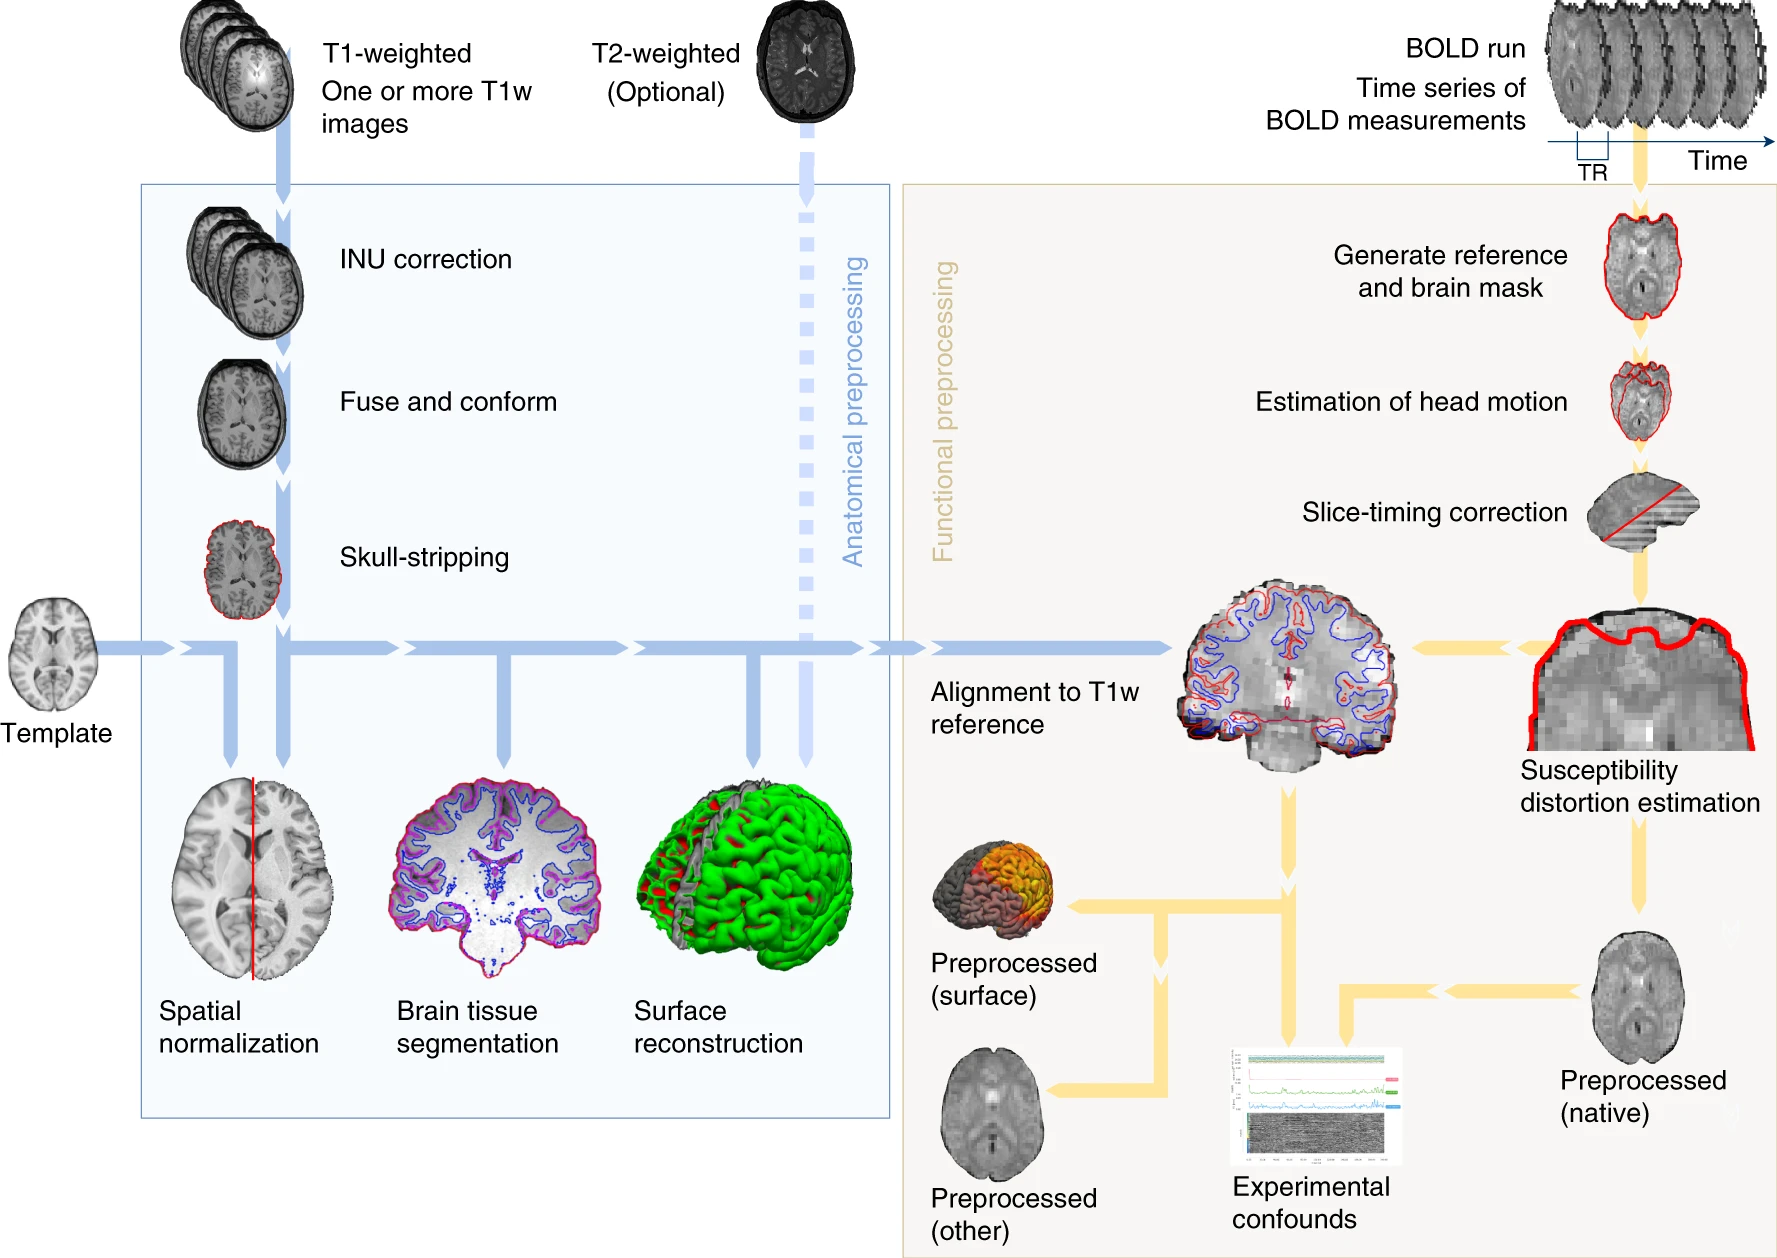
\includegraphics[width=\textwidth]{fMRIPrep_workflow.png}
	\caption{Preprocessing steps for structural and functional MRI data. (Taken from~\cite{Esteban2019-og})}
	\label{fig:fmri_workflow}
\end{figure}

While fMRI uses BOLD signal to capture data, dMRI exploits the magnetization of hydrogen in water molecules.
The water molecules diffuse at different rates depending on the tissue types, 
integrity, and architecture giving information about its direction and anisotropy~\cite{Soares2013-hw}.
This makes dMRI more suitable to study the neuronal function than blood-flow-based approach such as fMRI.
For example, to map brain connection or detect faulty connection of some psychiatric disorders~\cite{Le_Bihan2015-vp}.
Just like structural and functional MRI, dMRI acquisition is very sensitive to motion.
Correcting head motion is required during preprocessing.
Optionally, skull striping can also be performed to extract the brain data for analysis.
Dipy~\cite{Garyfallidis2014-ve} is a toolkit to perform these preprocessing techniques
on dMRI data and offers different modules to perform analysis and visualization of data.
Moreover, Dipy is integrated within the neuroimaging Python ecosystem.

The different MRI modalities presented in this section offer a non-intrusive way to study the brain.
However, they require multiple complex preprocessing steps before doing analysis of the data.
Lastly, a multitude of mature toolkit for preprocessing and analysis exist to process MRI data.


\section{Machine Learning applications} % 2
In recent years, machine learning (ML) methods have seen an increase interest 
accross multiple fields of application; neuroimaging is no exception.
While most ML techniques for neuroimaging lays in the analysis stage, some recent 
work tackle the problem of pre-processing using Deep Learning (DL).
Throughout this section, we will review some of the ML methods for analysing MRI 
data, their heavy usage motivating the development of a specific machine learning
framework for neuroimaging analysis, and recent work that use DL techniques to 
speed up current neuroimaging pipelines.

Using machine learning techniques to perform neuroimaging analysis is challenging.
Inherently, neuroimaging data contains few subjects (samples) and very large amounts
of voxels (often used as features).
The author in~\cite{Davatzikos2019-dc} says that, as of 2019, ML techniques used in
neuroimaging are not mature enough to be reliable in application.
However, a lot of efforts are put to overcome the current challenges in the field.
In a recent study~\cite{Mateos-Perez2018-wx}, the authors review ML applications on MRI data,
mainly structural, for both predicting clinical status or finding regions of interests (ROI)
for diseases and disorders.
Some of the applications presented include, but are not limited to: 
classification of Alzheimer's disease, diagnosis of Autism, automatic segmentation
of white matter lessions, or classification of the differents stages of Parkinson
and combinations of diseases with similar symptoms.
While obtening high accuracy is objectively desirable, in neuroimaging, it is much
more important to understand what are the major factors that influenced in making a prediction.
That is, understanding which features impact the prediction of some disease helps
in gaining knowledge on their biological implications.
This in part might explain the predominance of SVM in the analysis of neuromaging studies.
While ML methods are still growing in neuroimaging, they are invaluable in gaining 
a deeper understanding of the underlying biological aspects of diseases and disorders.

The joint combination of the increased prevalence, multiple methods, and unique 
challenges of machine learning methods in neuroimaging, motivates the development
of specific tools to perform ML analysis for neuroimaging.
The authors in~\cite{Abraham2014-zv} discuss the main steps performed for some 
neuroimaging analysis while using ML techniques.
In the same paper, the authors describe the main constructs used to develop
\textit{Nilearn}: A statistical analysis framework for neuroimaging in Python.
To name a few, Nilearn facilitates the steps to perform analysis by offering 
methods to perform data preparation such as reasmpling, signal cleaning, or data
visualization, decoding and encoding tools, and resting-state and functional connectivy analysis.
While such frameworks offers a multitude of tools to perform statistical analysis,
they still require pre-processing of the data, which is computatively demanding.

Thus far, the ML methods for neuroimaging that we discussed were only classic 
statistical methods, however, multiple DL techniques have also been studied.
In a recent review paper~\cite{Wen2018-to}, the authors discuss three applications
which can benefit from DL models.
In one paper reviewed~\cite{Nie2016-sw}, using features extracted from a CNN,
a SVM classified the lifetime of patients with brain tumors.
In another study~\cite{Wen2018-xm}, fMRI data related to data is interpreted using an auto-decoder.
Lastly, in~\cite{Zou2017-hd}, a 3D-CNN is used to classify ADHD.
While showing showing promising accuracy and fast inference time, training DL models
requires extensive training time and is prone to over-fitting; especially in the
setting of neuroimaging where the number of sample is low.

Two distinct parts of neuroimaging computing is the pre-processing steps and the analysis.
So far in this section, we only discussed the ML methods used for analysis due to
the large amount of studies using ML to perform neuroimaging analysis.
While few, there are some emerging efforts that propose using DL methods to speed up
the computation of the pre-processing steps.
With claisscal pre-processing pipeline being compute and time intensive, using 
DL techinques could significantly reduce the pre-processing time of neuroimaging studies
and bring more applications in clinics which requires results in a timely manner.
This motivated the development of FastSurfer~\cite{Henschel2020-vq}.
The authors of this framework develop novel methods to perform fast volumetric segmentation,
reconstruction of the cortical geometry, and estiamte the morphology of the brain.
While other tools use DL to solve specific problem of the pre-processing pipeline,
FastSurfer is a whole framework that allows complete pre-processing replicating the 
FreeSurfer framework.
The authors claim that ``despite being despite being orders of magnitude \textit{faster} than
traditional approaches, FastSurfer increases \textit{reliability and sensitivity}'' compared to FreeSurfer.
FreeSurfer generally takes \SI{7}{\hour} for a complete pre-processing pipeline, while
FastSurfer only takes approximately \SI{3.7}{\hour}; with only \SI{1}{\minute} of
processing time required to perform volumetric segmentation for both the cortical and subcortical regions.
This introduce the potential to perform studies on larger datasets and enables more
applications where segmentation processing time is needed.

With the many efforts put into developping ML techniques for neuroimaging, they 
became an intrisic part of the field.
The numerous applications and the complex challenges related to neuroimaging 
motivated the development of frameworks specific to the domain, such as Nilearn.
Furthermore, more recent work use DL models to increase either, or both, of accuracy
and processing speed for pre-processing and analysis.
While some challenges remain, the current integration of ML models into neuroimaging
shows promising results for better understanding of the biological implications from 
brain activation, coducting study on larger datasets, and increase the 
applicatibility where results are needed imminently.

\section{Reduced precision for neuroimaging} % 1-2
% TODO
% !! Mention of regularization methods and other smoothing techniques.
% !! IMPORTANT describe the state of neuroimaging problems. That is, they don't have
%  ground truth. So although two pipeline give different results, that does not
%  mean that one has to be wrong. 
% ? Mention the paper that reduce float64 to int32 for their experiments.
% !! Reduce precision could have similar effect as regularization or other smoothing techniques.
